\documentclass[dvipdfmx]{jsarticle}

\title{個人レベルでGithubを使う}
\author{Seiichi Nukayama}
\date{2021-07-09}
\usepackage{tcolorbox}
\usepackage{color}
\usepackage{listings, plistings}

% Java
\lstset{% 
  frame=single,
  backgroundcolor={\color[gray]{.9}},
  stringstyle={\ttfamily \color[rgb]{0,0,1}},
  commentstyle={\itshape \color[cmyk]{1,0,1,0}},
  identifierstyle={\ttfamily}, 
  keywordstyle={\ttfamily \color[cmyk]{0,1,0,0}},
  basicstyle={\ttfamily},
  breaklines=true,
  xleftmargin=0zw,
  xrightmargin=0zw,
  framerule=.2pt,
  columns=[l]{fullflexible},
  numbers=left,
  stepnumber=1,
  numberstyle={\scriptsize},
  numbersep=1em,
  language={Java},
  lineskip=-0.5zw,
  morecomment={[s][{\color[cmyk]{1,0,0,0}}]{/**}{*/}},
}
\usepackage{url}
% \usepackage[dvipdfmx]{graphicx}
\usepackage[dvipdfmx]{hyperref}
\usepackage{amsmath, amssymb}
\usepackage{itembkbx}
\usepackage{eclbkbox}	% required for `\breakbox' (yatex added)
\usepackage{enumerate}
\usepackage{setspace}
\fboxrule=0.5pt
\parindent=1em
\begin{document}

%\anaumeと入力すると穴埋め解答欄が作れるようにしてる。\anaumesmallで小さめの穴埋めになる。
\newcounter{mycounter} % カウンターを作る
\setcounter{mycounter}{0} % カウンターを初期化
\newcommand{\anaume}[1][]{\refstepcounter{mycounter}{#1}{\boxed{\phantom{aa}\themycounter \phantom{aa}}}} %穴埋め問題の空欄作ってる。
\newcommand{\anaumesmall}[1][]{\refstepcounter{mycounter}{#1}{\boxed{\tiny{\phantom{a}\themycounter \phantom{a}}}}}%小さい版作ってる。色々改造できる。

%% 修正時刻: Fri Jul  9 12:01:07 2021


\section{Eclipseで Github を使う}

\subsection{ワークスペースをGitで管理する}

\subsubsection{ワークスペース名の決定}

\textsf{C:}ドライブの直下にワークスペースを作成し、それをGitで管理することにする。

ワークスペース名: \textsf{workspace\_git}

\subsubsection{Githubでリポジトリを作成する}

Githubにサインインして、新しいリポジトリを作成する。

% 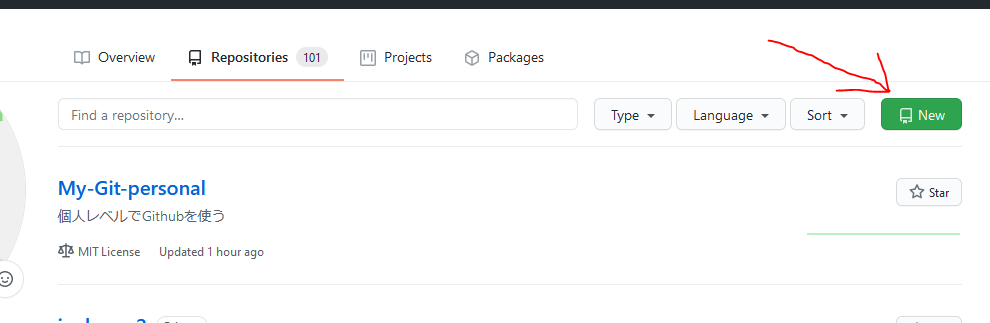
\includegraphics[width=10cm]{img/11newRepo.png}

\textsf{NEW}をクリックして始める。

\textsf{Create a new repository} の画面が開く。

\fbox{\textsf{Repository name}}

まず、リポジトリ名を入力する。今回は \textsf{workspace\_git} とした。

Description には、このリポジトリの簡単な説明を入れておく。
今回は、「git用ワークスペース」としておく。

% 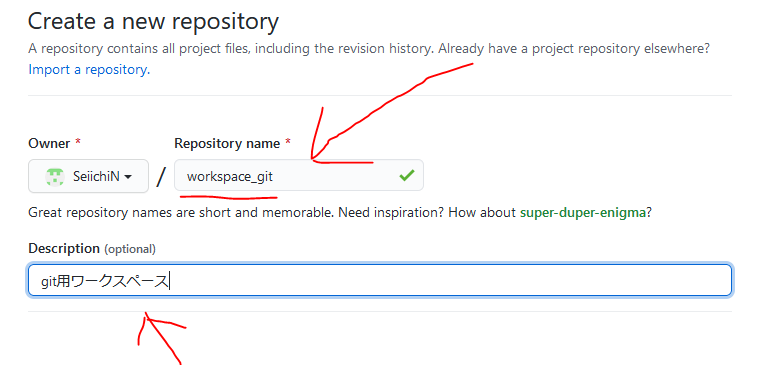
\includegraphics[width=10cm]{img/12repoName.png}

\fbox{\textsf{Public / Private}}

このリポジトリを公開するかどうかを設定する。今回は \textsf{Private} とする。

\fbox{\textsf{Add a README fle}}

README.md というファイルを作成するかどうかだが、作成しておいたほうが何かと便利。

\fbox{\textsf{Add .gitignore}}

.gitignore というファイルを作成するかどうかだが、これも作成しておいたほうが便利。

これにチェックを入れると、入力欄が表示される。ここでは \textsf{Java} を選択しておく。

\fbox{\textsf{Choose a license}}

どういうライセンスにするかを選択できる。今回は Private すなわち非公開なので、
選択しなくてもかまわない。

ちなみに一番ゆるいライセンスは、MITライセンス。

\fbox{\textsf{Create repository}} ボタンをクリックすると、リポジトリが作成される。

新しくできたリポジトリの画面が表示される。\fbox{Code} ボタンをクリックする。

\textsf{https://github.com/xxxxxx/workspace\_git.git} が表示されるので、
コピーしておく。(コピーボタンがあるので、それをクリック)


\subsubsection{クローンする}

今回は、C:ドライブ直下に Git用ワークスペースを作成したいので、
C:ドライブで コマンドプロンプトを開く。

\verb!C:> ! と表示されるので、\textsf{git clone } と入力してから、
Ctrl-v として、先ほどコピーしておいたものを貼り付ける。

\verb!C:> git clone https://github.com/xxxxxx/workspace_git.git!

これで、C:ドライブに \textsf{workspace\_git} というフォルダが作成されている。

\subsubsection{Eclipseでそのワークスペースで作業する}

Eclipseを起動して、その今作成したワークスペースを指定する。

そして、そこで何らかのプロジェクトを作成し、コードを書く。

今回は、\textsf{sample} という Javaプロジェクトを作成し、
\textsf{src} に \textsf{Main.java} というクラスを作成して、
以下のコードを書いた。

\begin{lstlisting}[caption=Main.java]
public class Main {
  public static void main(String[] args) {
    System.out.println("テスト");
  }
}
\end{lstlisting}

\subsubsection{ワークスペースの変更をGithubに反映させる}

\verb!C:\workspace_git! でコマンドプロンプトを開く。

\begin{tcolorbox}
 \verb!C:\workspace_git> git status!
\end{tcolorbox}

とする。

\begin{verbatim}
C:\workspace_git>git status
On branch main
Your branch is up to date with 'origin/main'.

Changes not staged for commit:
  (use "git add <file>..." to update what will be committed)
  (use "git restore <file>..." to discard changes in working directory)
        modified:   .gitignore

Untracked files:
  (use "git add <file>..." to include in what will be committed)
        sample/

no changes added to commit (use "git add" and/or "git commit -a")    
\end{verbatim}

\verb!git status -u!

とすると、フォルダのなかのファイルも表示してくれる。

\begin{verbatim}
C:\workspace_git>git status -u
On branch main
Your branch is up to date with 'origin/main'.

Changes not staged for commit:
  (use "git add <file>..." to update what will be committed)
  (use "git restore <file>..." to discard changes in working directory)
        modified:   .gitignore

Untracked files:
  (use "git add <file>..." to include in what will be committed)
        sample/.classpath
        sample/.project
        sample/.settings/org.eclipse.jdt.core.prefs
        sample/src/sample/Main.java

no changes added to commit (use "git add" and/or "git commit -a")    
\end{verbatim}


\end{document}

%% 修正時刻: Sat May  2 15:10:04 2020


%% 修正時刻: Fri Jul  9 14:15:28 2021
